\documentclass[10pt]{article}

\usepackage{amsthm}
\usepackage{amsmath}
\usepackage{amssymb}
\usepackage{mathtools}
\usepackage{graphicx}
\usepackage[colorinlistoftodos]{todonotes}
\usepackage{url}
\usepackage{xcolor}
\usepackage[font=small,labelfont=bf]{caption}

\usepackage{pgfplots}

\usepackage[left = 1cm, top = 1cm, bottom = 2cm, right = 1cm, nohead, nofoot]{geometry}

\pgfplotsset{width=20cm, compat=1.9}

\newcommand{\C}{\mathbb{C}}  % Complex
\newcommand{\R}{\mathbb{R}}  % Real
\newcommand{\Z}{\mathbb{Z}}  % Integers
\newcommand{\N}{\mathbb{N}}  % Naturals

\newcommand{\A}{\mathbb{A}}
\newcommand{\K}{\mathbb{K}}

\title{$\A$dvanced $\C$alculus}
\author{$\C$ason $\K$onzer}
\date{November 28, 2021}



\begin{document}
\maketitle

\newpage

%%%%%%%%%%%%%%%%%%%%%%%%%%%%%%%%%%%%%%%%%%%%%%%%%%%%%%%%%%%%%%%%%%%%%%%%%%%%%%%%%%%%%%%%%%%%%%%%
%%%%%%%%%%%%%%%%%%%%%%%%%%%%%%%%%%        Problem #1       %%%%%%%%%%%%%%%%%%%%%%%%%%%%%%%%%%%%%
\section{\underline{}}
\label{sec: Problem 1}

\noindent
Find the general solution of $ u_{xx} - 6u_{xy} + 9u_{yy} = 0 $ by the following: 
let $ x = v $ and $ y = w - 3v $, or equivalently, $ v = x $ and $ w = y + 3x $; 
define $ U(v,w) $ to be $ U(v,w) = u(v,w-3v) = u(x,y) $; 
derive and solve a PDE for $ U(v,w) $; 
convert back to $ u(x,y) $. 
Hint: the solution will involve two arbitrary functions. 
Use your solution to provide a non-trivial example of a solution. \\
\vspace{2.5mm}

\hrule 

\vspace{7.5mm}

\begin{itemize}
    \item Solve the characteristic $ B^2 - 4AC $.
    \subitem $ A = 1 $
    \subitem $ B = -6 $
    \subitem $ C = 9 $
    \subitem $ (-6)^2 - 4(1)(9) = 36 - 36 = 0 $
    \subsubitem The characteristic is parabolic $ \Rightarrow  $ Tartget $ U_{vv} = 0 $
    \item Solve for the partials.
    \subitem $ U_{v} = U_{x}x_{v} + U_{y}y_{v} $
    \subsubitem $ = U_{x} - 3U_{y} $
    \subitem $ U_{vv} = (U_{x} - 3U_{y})_{x}x_{v} + (U_{x} - 3U_{y})_{y}y_{v} $
    \subsubitem $ = (U_{xx} - 3U_{yx}) - 3(U_{xy} - 3U_{yy}) $
    \subsubitem $ = U_{xx} - 6U_{xy} + 9U_{yy} = 0 $
    \item Solve for U.
    \subitem $ U_{v} = j(w) + C $
    \subitem $ U = j(w)v + k(w) + C $
    \subitem $ u = j(y + 3x)x + k(y + 3x) + C $
    \item Example non-trivial solution.
    \subitem $ u = \sin(y + 3x)x + e^{y + 3x} $
    \subitem $ u_{x} = 3\cos(y + 3x)x + \sin(y + 3x) + 3e^{y + 3x} $
    \subitem $ u_{xx} = -9\sin(y + 3x)x + 3\cos(y + 3x) + 3\cos(y + 3x) + 9e^{y + 3x} = -9\sin(y + 3x)x + 6\cos(y + 3x) + 9e^{y + 3x} $
    \subitem $ u_{xy} = -3\sin(y + 3x)x + \cos(y + 3x) + 3e^{y + 3x} $
    \subitem $ u_{y} = \cos(y + 3x)x + e^{y + 3x} $
    \subitem $ u_{yy} = -\sin(y + 3x)x + e^{y + 3x} $
    \item Solving the non-trivial solution.
    \subitem $ (-9\sin(y + 3x)x + 6\cos(y + 3x) + 9e^{y + 3x}) - 6(-3\sin(y + 3x)x + \cos(y + 3x) + 3e^{y + 3x}) + 9(-\sin(y + 3x)x + e^{y + 3x}) $
    \subitem $ -9\sin(y + 3x)x + 6\cos(y + 3x) + 9e^{y + 3x} + 18\sin(y + 3x)x - 6\cos(y + 3x) - 18e^{y + 3x} - 9\sin(y + 3x)x + 9e^{y + 3x} $ 
    \subitem $ (18\sin(y + 3x)x - 18\sin(y + 3x)x) + (6\cos(y + 3x) - 6\cos(y + 3x)) + (18e^{y + 3x} - 18e^{y + 3x}) = 0 $ 
\end{itemize}

\newpage

%%%%%%%%%%%%%%%%%%%%%%%%%%%%%%%%%%%%%%%%%%%%%%%%%%%%%%%%%%%%%%%%%%%%%%%%%%%%%%%%%%%%%%%%%%%%%%%%
%%%%%%%%%%%%%%%%%%%%%%%%%%%%%%%%%%        Problem #2       %%%%%%%%%%%%%%%%%%%%%%%%%%%%%%%%%%%%%
\section{\underline{}}
\label{sec: Problem 2}

\noindent
Find the Fourier series representation of $ u(x,t) $, 
the solution to the heat equation on a metal bar of length $ L = 10 $ 
with $ \rho = 10.6 $, $ K = 1.04 $, $ \sigma = 0.056 $, and $ u(x,0) = f(x) = 4 - 0.8|x-5| $ 
on $ 0 \le x \le 10 $, extended as an odd function. 
Enforce the Dirichlet boundary condition of $ u(0,t) = u(10,t) = 0 $. \\
\vspace{2.5mm}

\hrule 

\vspace{7.5mm}

\begin{itemize}
    \item Solve for $ c = \dfrac{K}{\rho\sigma} $ and $ \lambda_{n} = \dfrac{cn\pi}{L} $.
    \subitem $ c = \dfrac{1.04}{10.6*0.056} = 1.7520 $
    \subitem $ \lambda_{n} = \dfrac{1.7520n\pi}{10} = 0.1752\pi n $
    \item Solve for $ \displaystyle B_{n} = \dfrac{2}{L} \int_{0}^{L} f(x) \sin{\dfrac{n\pi x}{L}} \,dx $
    \subitem $ \displaystyle B_{n} = \dfrac{2}{10} \int_{0}^{10} (4 - 0.8|x-5|) \sin{\dfrac{n\pi x}{10}} \,dx $
    \subitem $ \displaystyle B_{n} = \dfrac{1}{5} \Bigl[ \int_{0}^{5} (4 - 0.8(5-x)) \sin{\dfrac{n\pi x}{10}} \,dx + \int_{5}^{10} (4 - 0.8(x-5)) \sin{\dfrac{n\pi x}{10}} \,dx \Bigr] $
    \subitem $ \displaystyle B_{n} = \dfrac{1}{5} \Bigl[ \int_{0}^{5} (4 -4 + 0.8x) \sin{\dfrac{n\pi x}{10}} \,dx + \int_{5}^{10} (4 + 4 - 0.8x) \sin{\dfrac{n\pi x}{10}} \,dx \Bigr] $
    \subitem $ \displaystyle B_{n} = \dfrac{1}{5} \Bigl[ \int_{0}^{5} 0.8x\sin{\dfrac{n\pi x}{10}} \,dx + \int_{5}^{10} 8\sin{\dfrac{n\pi x}{10}} \,dx - \int_{5}^{10} 0.8x\sin{\dfrac{n\pi x}{10}} \,dx \Bigr] $
    \subitem $ \displaystyle B_{n} = \dfrac{1}{5} \Bigl[ \dfrac{0.8(10^2\sin{\dfrac{n\pi x}{10}} - 10\pi x\cos{\dfrac{n\pi x}{10}})}{n^2\pi^2} \Big|_{0}^{5} + \dfrac{80\cos{\dfrac{n\pi x}{10}}}{n\pi} \Big|_{5}^{10} - \dfrac{0.8(10^2\sin{\dfrac{n\pi x}{10}} - 10\pi x\cos{\dfrac{n\pi x}{10}})}{n^2\pi^2} \Big|_{5}^{10} \Bigr] $
    \subitem $ \displaystyle B_{n} = \dfrac{4}{25} \Bigl[ \dfrac{100\sin{\dfrac{n\pi}{2}}}{n^2\pi^2} + \dfrac{100\cos{n\pi}}{n\pi} + \dfrac{100\pi\cos{n\pi}}{n^2\pi^2} + \dfrac{100\sin{\dfrac{n\pi}{2}}}{n^2\pi^2} \Bigr] $
    \subitem $ \displaystyle B_{n} = \dfrac{400}{25} \Bigl[ \dfrac{\sin{\dfrac{n\pi}{2}}}{n^2\pi^2} + \dfrac{\cos{n\pi}}{n\pi} + \dfrac{\pi\cos{n\pi}}{n^2\pi^2} + \dfrac{\sin{\dfrac{n\pi}{2}}}{n^2\pi^2} \Bigr] $
    \subitem $ \displaystyle B_{n} = \dfrac{16}{n^2\pi^2} \Bigl[ 2\sin{\dfrac{n\pi}{2}} + (n + 1)\pi\cos{n\pi} \Bigr] $
    \item Under the given boundary condition we know the form of $ u_n $ and $ u $.
    \item Substitute $ B_{n}, L, \lambda_{n} $ into $ \displaystyle u_{n} =  B_{n}\sin{\dfrac{n\pi x}{L}}e^{-\lambda_{n}^{2}t}$
    \subitem $ \displaystyle u_{n} = \dfrac{16}{n^2\pi^2} \Bigl[ 2\sin{\dfrac{n\pi}{2}} + (n + 1)\pi\cos{n\pi} \Bigr]\sin{(\dfrac{n\pi x}{10})}e^{-0.0307\pi^2n^{2}t}$
    \item Substitute $ u_n $ into $ \displaystyle u = \sum_{n = 1}^{\infty} u_{n} $
    \subitem $ \displaystyle u = 16\sum_{n = 1}^{\infty} \dfrac{2\sin{(\dfrac{n\pi}{2})} + (n + 1)\pi\cos{(n\pi)}}{n^2\pi^2} \sin{(\dfrac{n\pi x}{10})}e^{-0.0307\pi^2n^{2}t}$
    \item With $ x = 0 $ and $ x = 10 $
    \subitem $ \displaystyle u(x=\{0,10\},t=t) = 16\sum_{n = 1}^{\infty} 0 = 0 $
\end{itemize}

\newpage

%%%%%%%%%%%%%%%%%%%%%%%%%%%%%%%%%%%%%%%%%%%%%%%%%%%%%%%%%%%%%%%%%%%%%%%%%%%%%%%%%%%%%%%%%%%%%%%%
%%%%%%%%%%%%%%%%%%%%%%%%%%%%%%%%%%        Problem #3       %%%%%%%%%%%%%%%%%%%%%%%%%%%%%%%%%%%%%
\section{\underline{}}
\label{sec: Problem 3}

\noindent
Use Mathematica and your solution from the last problem to plot $ u(x,0) $ and $ u(x,2) $ on the same graph. 
When defining $ u $, use the first four non-zero terms of the series.  \\
\vspace{2.5mm}

\hrule 

\vspace{7.5mm}

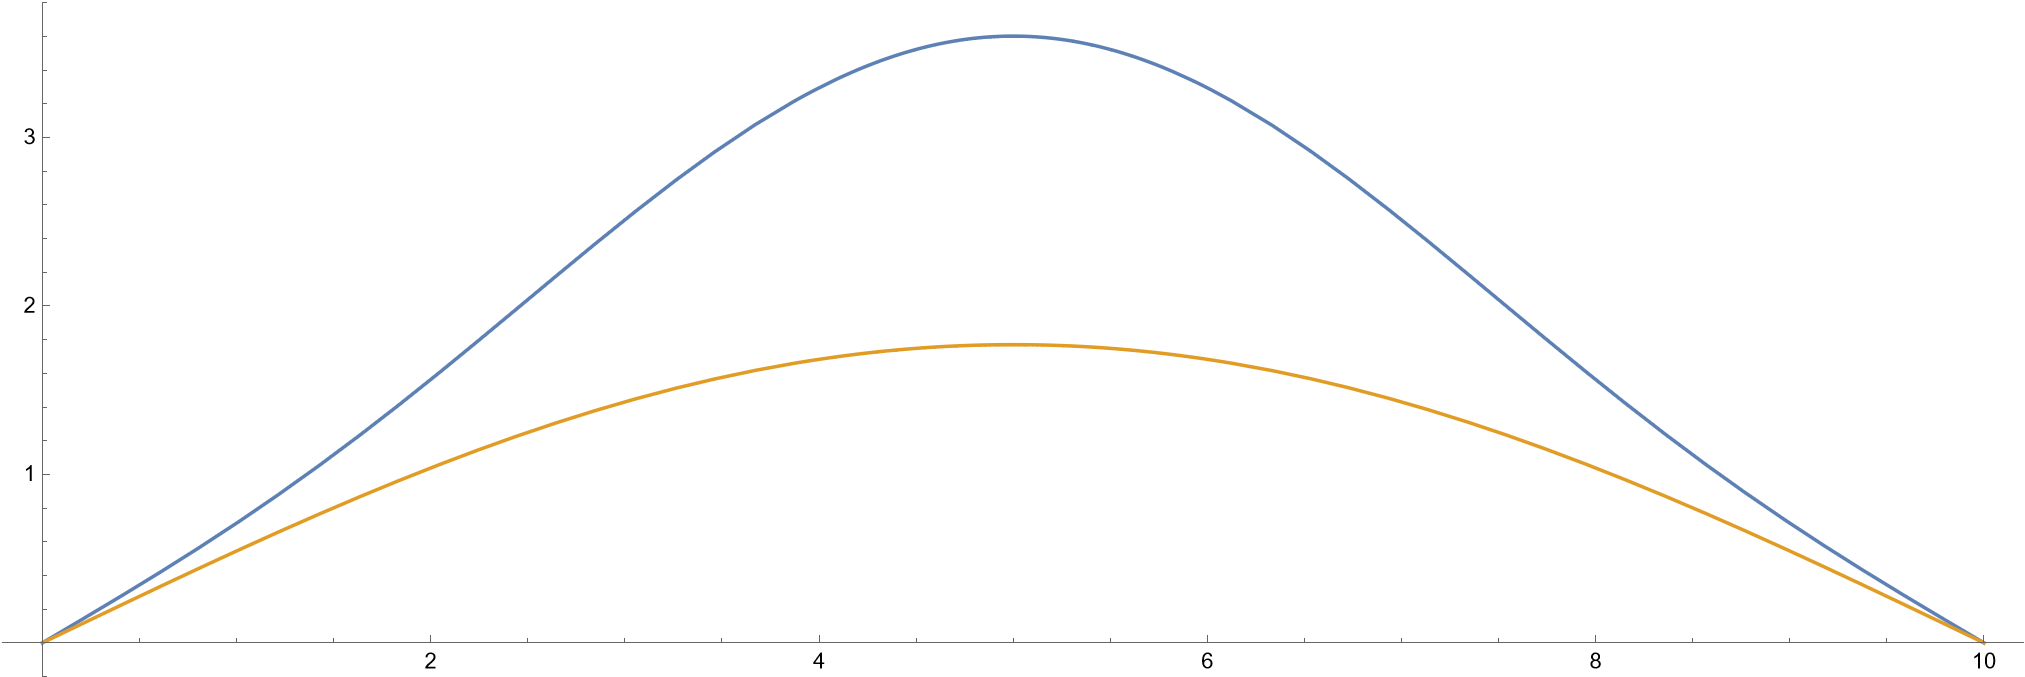
\includegraphics[width=\textwidth]{3.png}

\newpage

%%%%%%%%%%%%%%%%%%%%%%%%%%%%%%%%%%%%%%%%%%%%%%%%%%%%%%%%%%%%%%%%%%%%%%%%%%%%%%%%%%%%%%%%%%%%%%%%
%%%%%%%%%%%%%%%%%%%%%%%%%%%%%%%%%%        Problem #4       %%%%%%%%%%%%%%%%%%%%%%%%%%%%%%%%%%%%%
\section{\underline{}}
\label{sec: Problem 4}

\noindent
Find the Fourier series representation of the steady-state solution $ u(x,y) $ 
of the heat equation on the square metal plate with corners $ (0,0) $ and $ (2,2) $ 
in the plane, satisfying the following boundary conditions: 
$ u_y(x,0) = u_x(0,y) = u_x(2,y) = 0 $ and $ u(x,2) = \pi $. \\
\vspace{2.5mm}

\hrule 

\vspace{7.5mm}

\begin{itemize}
    \item Solve for $ p_{n} =\dfrac{n\pi}{a} $
    \subitem  $ p_{n} =\dfrac{n\pi}{2} $
    \item Solve for $ \displaystyle a_{0} =\dfrac{1}{a} \int_{0}^{a} f(x) \,dx $
    \subitem $ \displaystyle a_{0} =\dfrac{1}{2} \int_{0}^{2} \pi \,dx = \dfrac{1}{2} \Bigl[ \pi x \Big|_{0}^{2} \Bigr] = \dfrac{1}{2} \Bigl[ 2\pi - 0\Bigr] $
    \subitem $ a_{0} = \pi = A_{0} $
    \item Solve for $ \displaystyle a_{n} =\dfrac{2}{a} \int_{0}^{a} f(x)\cos{\dfrac{n\pi x}{a}} \,dx $
    \subitem $ \displaystyle a_{n} = \dfrac{2}{2} \int_{0}^{2} \pi\cos{\dfrac{n\pi x}{2}} \,dx = \dfrac{2\sin{\dfrac{n\pi x}{2}}}{n} \Big|_{0}^{2} = \Bigl[ \dfrac{2\sin{n\pi}}{n} - 0 \Bigr] $
    \subitem $ \displaystyle a_{n} = 0 = A_{n}(e^{p_{n}y} - e^{-p_{n}y}) = A_{n} $
    \item Under the given boundary condition we know the form of $ u $.
    \item Substitute $ A_{0}, A_{n}, L, p_{n} $ into $ \displaystyle u =  A_{0} + \sum_{n = 1}^{\infty} A_{n}\cos{(p_{n}x)}\Bigl[ e^{p_{n}y} - e^{-p_{n}y} \Bigr] $
    \subitem $ \displaystyle u =  \pi + \sum_{n = 1}^{\infty} 0 $
    \subitem $ \displaystyle u(x,y) =  \pi  $
\end{itemize}

\newpage

\end{document}


%%%%%%%%%%%%%%%%%%%%%%%%%%%%%%%%%%%%%%%%%%%%%%%%%%%%%%%%%%%%%%%%%%%%%%%%%%%%%%%%%%%%%%%%%%%%%%%%
%%%%%%%%%%%%%  Comments - November 13, 2021 Advanced Calculus Written Home Work #7  %%%%%%%%%%%%%